% !TeX root = ../main.tex

\chapter{实验设计与结果分析}

本章在第二章与第三章的研究内容的基础上,进行对代码克隆方法的实验实现与评估,对实证研究的具体结果分析。在基于抽象语法树的代码克隆方法中,本文以来自StackOverflow的代码片段与来自Etherscan的开源智能合约项目作为输入,提取其中合约与函数;对每一个来自StackOverflow的合约或者函数,寻找它对应的代码克隆对。在第三章的实证研究部分,本文描述了本文使用代码克隆寻找StackOverflow漏洞与低效模式的实验方法。

本文的研究问题如下所示:

 \textbf{研究问题一:BLEU能够判断代码相似?}BLEU可以作为一种代码片段相似的评价指标,本问题探究了直接使用BLEU的效果,并且建立了验证数据集。

\textbf{研究问题二: 代码克隆方法能否找到漏洞与Gas低效模式一致的代码克隆对?}本问题探究了其他在智能合约常用的代码克隆方法在漏洞与Gas低效模式定位一致的有效性。

%\textbf{研究问题三: 代码克隆方法能够找到漏洞与Gas低效模式定位一致的克隆对?}本文检测了在匹配区域存在漏洞与Gas低效模式的匹配对,进行手动验证,并且对结果进行分析。

%\item \textbf{研究问题4}: 代码克隆方法能够找到Gas低效模式定位一致的克隆对?
\textbf{研究问题三: 在StackOverflow中存在多少漏洞?}本文从合约与函数的角度进行了检测,展示了代码克隆方法在StackOverflow的漏洞层面的结果,探究了被接受答案的安全性。

\textbf{研究问题四: 在StackOverflow中存在多少Gas低效模式?}本文展示了StackOverflow上存在的Gas低效模式,并且分析了Gas低效模式的Gas消耗估计。

\textbf{研究问题五: 来自StackOverflow的漏洞与Gas低效模式在开源智能合约中的普遍程度?}本文探究了StackOverflow上的漏洞与Gas低效模式出现在开源项目的可能频率。探究同时在StackOverflow出现的、最有可能扩散的漏洞与Gas低效模式类型。

本文首先描述了本文实验的数据大小,然后是各项研究问题。

其中研究问题一到研究问题三用于验证代码克隆方法是否真的能够在保证语法一致,语义相似的情况下,确定漏洞定位一致、Gas低效模式定位一致的代码克隆对。

在研究问题四到研究问题六本文对StackOverflow的漏洞与Gas低效模式的分布以及在开源智能合约中的扩散分布进行探究。

\section{开源项目与问答网站实验数据}

本文爬取了Etherscan的开源项目,并且提取了合约和函数。本文总共爬取在2021 年 10 月 20 日之前发布了 176,324 个开源项目,包含 554,806 个智能合约和 1,128,473 个函数。这些开源项目的平均代码行数为497,56行,其中91.6\%的代码不超过1,000行,共计87,633,028行。

本文不需要重复的合约与函数,因此本文对合约与函数去重,去重后一个合约或函数可能来自多个开源项目,本文同样保存了这个信息。这种去重是根据Token序列完成的,此时本文要求仅Token序列完全一致时是重复的。删除重复后,共有 69,322 个不同的合约与123,287 个函数。

%去除重复后的数据集将在 研究问题1 到 研究问题4 中用于匹配对分析和错误检测,而关于扩散的分析则使用第三章描述的重用方法检测。

从 StackOverflow 上的所有帖子中获取代码片段,也处理成合约与函数的形式。

本文爬取了自 2020 年 11 月到 2021 年 1 月 在 StackOverflow 上所有关于智能合约的帖子,总计32,258条帖子,并提取了 HTML 语言中带有标签 $<$code$>$ 的元素的内容。共有 9,787 个帖子存在代码片段,它们包含 91,654 个不可编译的合约和 236,184 个不可编译的函数。每个帖子的平均代码行数为 134.55 行,总共 1,316,840 行。使用与开源项目同样的逻辑去除重复后,有 9,631 个合约和 6,339 个函数。表\ref{dataset} 显示了这两个数据集的统计信息。

\begin{table*}[]%dataset
\centering

\begin{tabular}{c c c c c c c c}
\hline
                         & {\color[HTML]{494949} }                        & \multicolumn{2}{c}{行数} & \multicolumn{2}{c}{{\color[HTML]{494949} 去重前}} & \multicolumn{2}{c}{去重后} \\ \cmidrule(r){3-4}  \cmidrule(r){5-6} \cmidrule{7-8} 
\multirow{-2}{*}{来源} & \multirow{-2}{*}{{\color[HTML]{494949} 总计}} & 平均    & 总计         & 合约                      & 函数                      & 合约          & 函数          \\ \hline
开源项目           & 176,324                                        & 497.56     & 87,633,028    & 554,806                        & 1,128,473                      & 69,322             & 130,287            \\ %\hline
StackOverflow          & 9,787                                          & 134.55     & 1,316,840     & 91,654                         & 236,184                        & 9,631              & 6,339              \\ \hline
\end{tabular}
\caption{数据集统计}
\label{dataset}
\end{table*}

\subsection{对比方法}
代码克隆方法能够检测类型一、类型二与类型三的代码克隆;其中,由于类型一的代码克隆是完全相同的代码克隆对,因此本文的对比针对类型二与类型三的方法。

目前已有的代码克隆方法中,能够支持语言层面扩展的方法较少,根据智能合约领域相关论文\cite{smartembed}\cite{clone_esystem},本文发现目前较为常用的方法是NICAD\cite{nicad}与CCFinder\cite{clone4}。本文找到了NICAD的公开软件,对于CCFinder,本文并没有找到相关论文对CCFinder在智能合约实现的公开软件,同时CCFinder并不支持交叉克隆检测。

NICAD是一种基于Token的、使用解析和近似文本比较的代码克隆检测工具,在通过规范化、过滤或抽象,使用盲目或一致的重命名、过滤或抽象不相关的特征(如声明)的预处理步骤后,它使用优化的最长公共子序列(LCS)文本比较算法对提取和规范化的代码片段进行比较,以发现代码克隆对。通过对NICAD设置不同阈值,它能够检测到类型一、类型二、类型三的代码克隆。

NICAD 支持交叉克隆检测,即检测单个软件系统版本之间或跨不同软件系统的代码克隆,方法仅报告在两个版本或系统之间交叉的那些克隆。它使用允许轻松添加其他编程语言和粒度的插件架构。NICAD的特点使得它能够与本文的方法进行比较。

本文使用NICAD检测代码克隆类型二的默认设置与检测代码克隆类型三的默认设置,在后续的对比实验中,它们被分别称为NICAD2与NICAD3。

\subsection{验证数据集}

本文希望建立一个经过人工验证的与代码克隆方法无关的小型数据集用于后续基于抽象语法树方法的代码克隆方法的检验。
随机的选择数据组成匹配对是效率极低的,因为这些匹配对可能完全无关联,因此使用BLEU作为两个合约或函数的相似指标帮助本文筛选一部分克隆对。

本文的做法是:对于一个来自StackOverflow的合约或者函数,本文寻找它的BLEU取值高的来自开源项目的合约或者函数,以此作为一种可能正确的相似匹配对;本文对这些可能正确的相似匹配对进行多人共同进行的手动验证;本文总结了一种手动检验的规则,用于协同验证。

计算BLEU需要输入分割成数组形式的文本;本文对经过预处理,已经清除了注释与统一了代码格式的数据,根据空格进行分割,形成代码文本数组。

为了使人工验证更加客观,邀请了三名参与者来验证匹配对。在验证中,第一和第二参与者首先查看每个匹配对并总结出一套人工匹配规则,然后根据汇总规则将每个匹配对分为三种不同的类型,它们的依据如表\ref{rules}所示。分类结束后,由第三名参加者讨论并再次对两名参加者意见不一致的部分进行分类。

对于这三种类型的具体介绍如下:

\begin{enumerate}

  \item \textbf{相同语法、相同语义}: 属于该类型的匹配对在语法和语义上完全一致,命名为类型一。
  
  \item \textbf{相同语法、相似语义}:当代码的语法完全相同但语义不同时。这样的匹配对可能会为同一语句定义不同名称的变量,或者函数的参数名称不同。语法的一致性确保了出现在开源项目上的错误也可以出现在 StackOverflow 上的代码片段中。

  \item \textbf{不同语法、不同语义}:当一个匹配对不满足上述两个条件时,它会被归类为类型 3。它在语法和语义上不够相似,以至于这个匹配对对应的开源项目不能用于进一步的 漏洞与Gas低效模式 检测。

\end{enumerate}

\begin{table*}[]
\centering
\begin{tabular}{l l l}
\hline
{\color[HTML]{494949} 类型} & {\color[HTML]{494949} 描述}                           & {\color[HTML]{494949} 分类标准}   \\ \hline
{\color[HTML]{494949} 1}     & {\color[HTML]{494949} 相同语法,相同语义}           & {\color[HTML]{494949} (1) 相同的代码}    \\ \hline
{\color[HTML]{494949} 2} &
  {\color[HTML]{494949} 相同语法,相似语义} &
  {\color[HTML]{494949} \begin{tabular}[c]{@{}l@{}}(1) 不同合约名\\ (2) 不同变量名\\ (3) 相同变量名,不同变量值\\ (4) 有或没有emit\end{tabular}} \\ \hline
{\color[HTML]{494949} 3}     & {\color[HTML]{494949} 不同语法,不同语义} & {\color[HTML]{494949} (1) 其他情况} \\ \hline
\end{tabular}
\caption{人工验证规则}
\label{rules}
\end{table*}

% \begin{figure}[htbp]
% \centering
% 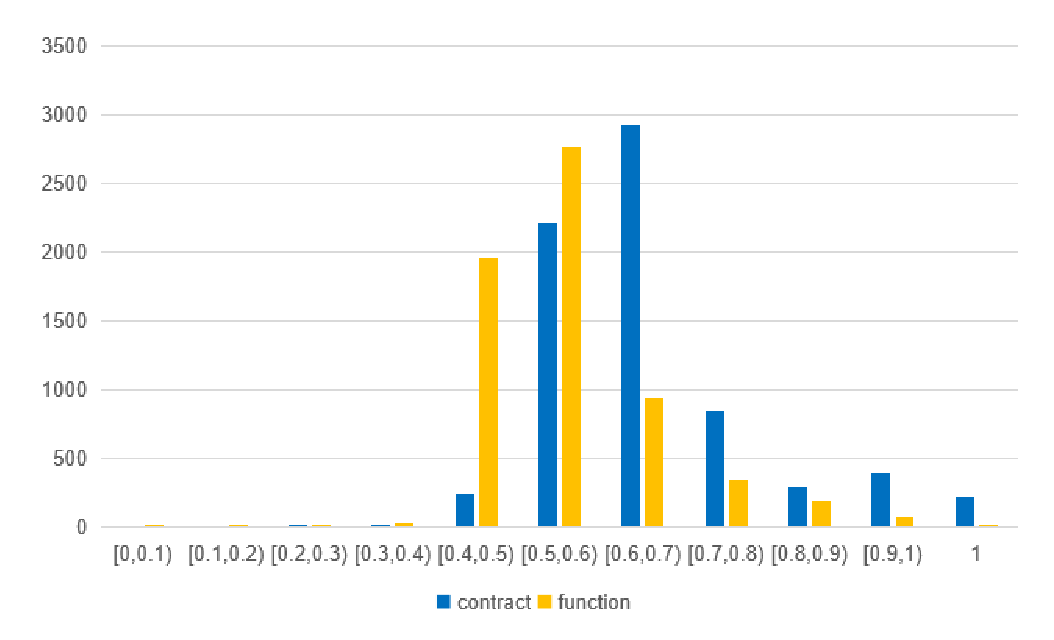
\includegraphics[width=0.8\textwidth]{figures/con_fun.eps}
% \caption{合约或函数匹配对的分布}
% \captionsetup{font={footnotesize}}
% \label{con_fun}
% %\vspace{-4mm}
% \end{figure}
%图 \ref{con_fun} 显示了匹配的合约或函数对的分布。

本文称属于类型一与类型二的匹配对为相似匹配对。最后,本文找到合约层面650对相似匹配对与函数层面118对函数匹配对。

\section{\label{snippet_clone}代码片段相似匹配实验设计与结果分析}

\textbf{研究问题一:BLEU 能够判断代码相似?}

虽然本文在第二章论述了BLEU如何帮本文找到语义相似的克隆对以及它在注释生成相关研究中是如何作为一种评估代码相似性的指标,但是本文仍然需要验证它的有效性。同时,本文也验证了直接使用BLEU,并且选择其中BLEU取值高的匹配对是否能够保证漏洞或Gas低效模式定位一致。

\begin{table}[htbp]
\centering
\begin{tabular}{@{}cccccc@{}}
\toprule
                    & 类型 & {[}0.7,0.8) & {[}0.8,0.9) & {[}0.9,1{]} & 总计  \\ \midrule
\multirow{3}{*}{合约} & 1  & 0           & 0           & 43          & 43  \\
                    & 2  & 69          & 213         & 325         & 607 \\ \cmidrule(l){2-6} 
                    & 总计 & 69          & 213         & 368         & 650 \\ \midrule
\multirow{3}{*}{函数} & 1  & 0           & 17          & 45          & 62  \\
                    & 2  & 0           & 47          & 9           & 56  \\ \cmidrule(l){2-6} 
                    & 总计 & 0           & 64          & 54          & 118 \\ \bottomrule
\end{tabular}
\caption{验证数据集在不同BLEU区间的相似匹配对分布}
\label{manual_result}
\end{table}

手动验证可以帮助本文找到相似匹配对。为了缩小手动验证的范围,本文选取阈值 BLEU 大于 0.7的匹配对,不同BLEU结果对代码相似程度的影响如图\ref{manual_result}所示。

在合约层面上,随着 BLEU 值的降低,类型 1 和类型 2 在匹配对中的比例也随之降低。

在函数层面上,来自 StackOverflow 的函数可能是 JavaScript 函数。当本文使用 JavaScript 函数从 开源项目库 中查找匹配对时,所有 JavaScript 函数的最高 BLEU 值为 0.57,低于 0.8。所以 JavaScript 函数被本文的 BLEU 阈值过滤掉。

从表\ref{manual_result}可以看出,合约层面,在区间 [0.9,1) 中,相似匹配对占 57\%,在 [0.8,0.9) 区间中为 33\%,[0.7,0.8)区间为10\%,共获得650对相似匹配对。
函数层面,在区间 [0.9,1) 中,相似匹配对占 46\%,在 [0.8,0.9) 区间中为 54\%,共获得118对相似匹配对。

综上所述,通过将 BLEU 阈值设置为 0.7,本文可以在合约和函数层面上分别获得共计650 个合约相似匹配对和 118 个函数匹配对。

BLEU在函数层面的效果较差,主要原因是函数的行数过短,导致两段代码差异较大时,仍然能获得较高的BLEU,但是代码克隆方法可以检测这些匹配对在语法层面的不一致。

可以发现,当匹配对作为文本的BLEU值越高,匹配对是相似匹配对的可能性越大,BLEU与相似匹配对呈现正相关;极高的BLEU也不代表它们能够找到漏洞与Gas低效模式定位一致的代码克隆对。

\textbf{研究问题二: 代码克隆方法能否找到漏洞与Gas低效模式一致的代码克隆对?}

在本节中,本文使用代码克隆方法自动化的寻找能够映射错误的代码克隆对;在研究问题一中,本文对BLEU取值在[0.7,1]的范围的相似匹配对抽样进行了人工检测,检测结果表明BLEU能够帮助本文找到语义相似的匹配对。

本文在收集的两个数据集中应用了代码克隆方法,取BLEU阈值0.7。本文得到了 1120 个合约代码克隆对和 609 个函数代码克隆对,它们来自1258个帖子,分别对应来自Etherscan 的 529 个和 396 个 开源项目,去除交集后,总共有730个开源合约。

% %查准分析
% 本文希望探究语法一致、语义相似的代码克隆对可以让出现在开源项目的漏洞或者低效模式一致的定位到与它互为克隆对的来自StackOverflow的合约或者函数。本文随机抽取了合约与函数层面各一百对克隆对进行手工验证;要求这些克隆对至少存在一个能够定位的漏洞或者低效模式。

% 对于一个漏洞,本文首先确定定位位置是否正确,也就是本文认为的克隆对是合约与合约的克隆或函数与函数的克隆。其次,本文检测这些漏洞与Gas低效模式是否正确的映射到StackOverflow的代码片段。

% 本文发现代码克隆方法在漏洞与Gas低效模式定位上,90\%(192/200)的合约层面克隆对与91\%的函数层面克隆对(182/200)都能够正确的定位。
% 对于NICAD2,它能够检测类型一与类型二的代码克隆,验证结果表明它的有效性在

% 考虑到本文寻找的是语法一致的克隆对,这种克隆对属于代码克隆中的类型二。它能够检测到非可执行元素(例如空格、制表符、注释等)、标识符名称、文字和类型名称的差异。尤其的,本文也要求变量类型一致,以保证多种涉及到变量类型的漏洞或Gas低效模式的一致性,实验证明本文的方法是有效的。

% %查全分析
% 由于本文对BLEU高的匹配对结果人工验证生成了验证数据集,因此本文希望通过对验证数据集的查全率表明本文方法的效果。

% 在合约层面,本文的1120个合约匹配对中找到了研究问题1中的144个相似匹配对中的141个,查全率为97.91\%。在函数层面,本文的609个函数匹配对找到了研究问题1中的52个匹配对中的51个,查全率为98.07\%。

% 这是由于人工检验的逻辑与本文的代码克隆方法是一致的;较高的查全率表明本文的方法能够找到语法一致、语义相似的克隆对。

%分析
本文的目标是找到能够保证漏洞与Gas低效模式定位一致的代码克隆对,这类似一个信息检索问题,本文可以使用查准率与查全率来验证本文的效果。

\begin{equation}
    \mbox{查全率}=\frac{\mbox{预测为真的样本}}{\mbox{实际为真的样本}}=\frac{TP}{TP+FN}   
\end{equation}

\begin{equation}
    \mbox{查准率}=\frac{\mbox{实际为真的样本}}{\mbox{预测为真的样本}}=\frac{TP}{TP+FP}
\end{equation}

本文希望探究语法一致、语义相似的代码克隆对可以让出现在开源项目的漏洞或者低效模式一致的定位到与它互为克隆对的来自StackOverflow的合约或者函数。本文随机抽取了合约与函数层面各一百对克隆对进行手工验证;要求这些克隆对至少存在一个能够定位的漏洞或者低效模式。
对于一个漏洞,本文首先确定定位位置是否正确。其次,本文检测这些漏洞与Gas低效模式是否正确的映射到StackOverflow的代码片段。

由于本文对BLEU高的匹配对结果人工验证生成了验证数据集,因此本文希望通过对验证数据集的查全率表明本文方法的效果。

结果如表\ref{recallCompare}所示,使用AST代指本文方法,可以发现,在克隆对数量上,本文方法在NICAD2与NICAD3之间。对于NICAD2方法,它的查准率极高然而查全率较低,仅为合约层面的41\%与函数层面的21\%,实际上,NICAD2的结果完全被验证数据集包含。对于NICAD3方法,它的查全率极高然而准确率较低,仅为合约层面的43\%与函数层面的52\%。由于本文的目标是验证StackOverflow上的漏洞与Gas低效模式分布与扩散分布,足够高的查准率能够保证后续验证的效果,同时与NICAD2相比,本文能够找到更多的克隆对,因此,本文认为在类型二与类型三的代码克隆上,本文的方法在当前任务上更加有效。同时,这也证明了本文的方法能够更好的定位到智能合约的漏洞与Gas低效模式。

在对NICAD2与NICAD3的验证过程中,本文发现NICAD一类的代码克隆检测方法在检测不同程度代码克隆时,无法准确的包含漏洞与Gas低效模式定位一致的代码克隆对。这是由于随着相似阈值的降低,更多的保证定位一致的代码克隆对与不能保证定位一致的代码克隆对都会增加。这使得克隆对的数量增加,然而有效性降低。这说明了NICAD不能区分能够保证漏洞与Gas低效模式定位一致的代码克隆对。

% %查准
% \begin{table}[htbp]
% \centering
% \caption{查准率比较结果}
% \begin{tabular}{@{}ccccc@{}}
% \toprule
% 查准率                 & 工具     & Bug   & Gas低效模式 & 总计& 克隆对数量     \\ \midrule
% \multirow{3}{*}{合约} & AST    & 91\%  & 89\%    & 90\% & 1120 \\
%                     & NiCad2 & 100\% & 100\%   & 100\%& 271 \\
%                     & NiCad3 & 53\%  & 33\%    & 43\%  & 2693\\ \midrule
% \multirow{3}{*}{函数} & AST    & 92\%  & 90\%    & 91\%  & 609 \\
%                     & NiCad2 & 100\% & 100\%   & 100\%  & 25 \\
%                     & NiCad3 & 97\%  & 85\%    & 52\% & 955  \\ \bottomrule
% \end{tabular}
% \label{precisionCompare}
% \end{table}

%查全
\begin{table}[]
\centering

\resizebox{\textwidth}{!}{%
\begin{tabular}{cccccccccc}
\hline
\multicolumn{1}{l}{\multirow{2}{*}{}} &
  \multirow{2}{*}{工具} &
  \multirow{2}{*}{克隆对数量} &
  \multirow{2}{*}{TP} &
  \multirow{2}{*}{FN} &
  \multirow{2}{*}{TP+FN} &
  \multirow{2}{*}{查全率} &
  \multicolumn{3}{c}{查准率} \\ \cline{8-10} 
\multicolumn{1}{l}{} &        &      &     &     &     &      & Bug   & Gas低效模式 & 总计    \\ \hline
\multirow{3}{*}{合约}  & AST    & 1120 & 637 & 13  & 650 & 98\% & 91\%  & 89\%    & 90\%  \\
                     & NICAD2 & 271  & 267 & 384 & 650 & 41\% & 100\% & 100\%   & 100\% \\
                     & NICAD3 & 2693 & 644 & 7   & 650 & 99\% & 53\%  & 33\%    & 43\%  \\ \hline
\multirow{3}{*}{函数}  & AST    & 609  & 116 & 2   & 118 & 98\% & 92\%  & 90\%    & 91\%  \\
                     & NICAD2 & 25   & 25  & 93  & 118 & 21\% & 100\% & 100\%   & 100\% \\ 
                     & NICAD3 & 955  & 107 & 11  & 118 & 91\% & 60\%  & 44\%    & 52\%  \\ \hline
\end{tabular}
}
\caption{查准率与查全率比较结果}
\label{recallCompare}
\end{table}


%实证研究结果
本文使用这三种工具对1120份项目进行了检查,其中453份有漏洞,占40.45\%;697份有Gas低效模式,占62.23\%,检测结果如表\ref{compliRes}所示。

有漏洞的项目平均存在4.96个漏洞,有低效模式的项目平均存在1.58个低效模式。观察检测结果本文可以发现,在漏洞方面,占据重要比例的漏洞是Arithmetic。在Gas低效模式方面是Pattern2。

Arithmetic指的是代码编写者编写的代码存在与计算有关的如上下溢出一类的问题,Pattern2指的是额外的变量类型转换操作使得Gas消耗增加。

本文随机抽取了100份存在Arithmetic漏洞的项目进行手动辨别,其中一半来自Mythril,另一半来自Osiris。当一个Arithmetic漏洞在某种输入下能够导致上下溢出,本文就判定为真漏洞。

\begin{table}[htb]\scriptsize%\footnotesize%
\centering
\begin{tabular}{l} 
\textbf{\tabincell{c}{开源项目 0x5e851c761fc6b8da67459a74f7e2849032473d1f}}: \\ 
\tabincell{l}{...\\ function receiveApproval(address from, uint256 tokens, address token, bytes data) public   \{ \\
  \quad  ERC20Interface(token).transferFrom(from, address(this), tokens);\\
  \quad  emit LogBytes(data);\\
 \}\\... }
\end{tabular}
\vspace{-2mm}
%\caption{receiveApproval函数}
%\label{example}
\end{table}


首先,对于Osiris而言,它在Arithmetic重要检测三类漏洞:上下溢出、截断与有符号向无符号转换错误。在50份由它检测的项目中,本文发现上下溢出是最重要的漏洞类型。对于Mythril而言,它仅检测上下溢出问题。

本文发现Myhtirl工具检测的Arithmetic漏洞准确率为84\%(42/50),Osiris工具准确率为86\%(43/50)。错误原因主要包括两点。

\begin{itemize}

    \item 存在漏洞定位错误以及代码与漏洞完全不相关的情况,例如它会检测到ERC20的transferFrom函数,并且标记它为上溢。
    \item 项目可能使用require或assert关键字避免Arithmetic漏洞,在较新的语言版本,这项功能一般通过safeMath库实现;然而本文发现部分使用safeMath库中的正确调用的代码仍然会被工具检测为漏洞,检查代码的其余使用了safeMath库的算术操作,本文认为一种可能的原因是工具将两层及以上嵌套mapping中的正确算术操作认定为漏洞。如下所示,mapping变量allowed类似Python语言中的字典,对于一个address的键,能够找到一个类型为mapping(address => uint256)的值。此时allowed总共为两层的mapping。
    
    \begin{table}[htbp]
    \centering
    \begin{tabular}{l} 
    \tabincell{l}{
    mapping (address => mapping (address => uint256)) internal allowed;
    }
    \end{tabular}
    \end{table}
    
\end{itemize}

%举一个代币合约的例子.
如图\ref{overflow-example}所示,由于第二行if语句的存在,第三行的下溢漏洞可能不被检测。编写者并没有在第四行对上溢情况做处理,这导致工具将其标为Arithmetic漏洞;这段代码存在于一个代币合约当中,代码的逻辑是对于指定的交易者,它将接收到变量amount指示数量的以太币,由于以太币的数量难以超过uint最大值,实际环境中并未因为这个上溢漏洞产生上溢事件。

代码中出现漏洞意味着错误的编程方式与代码最佳实践的缺失。

\begin{figure}[htbp]
\centering
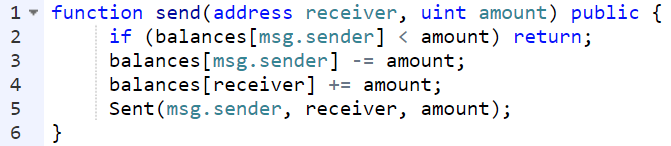
\includegraphics[width=0.8\textwidth]{figures/overflow-example.png}
\caption{存在上溢漏洞的例子}
\captionsetup{font={footnotesize}}
\label{overflow-example}
\end{figure}

\begin{table}[htbp]

\centering
\resizebox{\textwidth}{!}{%
\begin{tabular}{ccccccccc}
\hline
漏洞类型   & Access-Control & Arithmetic & Denial-Service & Reentrancy & Unchecked-Low-Calls & Front-Running & Time-Manipulation & 总计 \\ \hline
Mythril & 15  & 507  & 0  & 129 & 0   & 48 & 0   & 699  \\
Osiris  & 0   & 567  & 17 & 10  & 0   & 0  & 46  & 640  \\
Slither & 59  & 0    & 62 & 257 & 183 & 0  & 77  & 638  \\
总计      & 74  & 1074 & 79 & 396 & 183 & 48 & 123 & 1977 \\ \hline
低效模式类型 & Pattern1       & Pattern2   & Pattern3       & Pattern4   & Pattern5            & Pattern6      &                   & 总计 \\ \hline
总计      & 162 & 566  & 31 & 24  & 183 & 79 &     & 1045 \\ \hline
\end{tabular} 
}
\caption{开源项目的漏洞与Gas低效模式分布}
\label{compliRes}
\end{table}

% \textbf{研究问题三: 代码克隆方法找到了多少代码克隆对?}

% %完整的检测结果
% %假阳性 一致性
% 本文希望探究语法一致、语义相似的代码克隆对可以让出现在开源项目的漏洞或者低效模式一致的定位到与它互为克隆对的来自StackOverflow的合约或者函数。本文随机抽取了合约与函数层面各一百对克隆对进行手工验证;要求这些克隆对至少存在一个能够定位的漏洞或者低效模式。

% 对于一个漏洞,本文首先确定定位位置是否正确,也就是本文认为的克隆对是合约与合约的克隆或函数与函数的克隆。其次,本文检测这些危害是否正确的映射到StackOverflow的代码片段。

% 本文发现代码克隆方法在漏洞与Gas低效模式定位上,96\%(192/200)的合约层面克隆对与100\%的函数层面克隆对(200/200)都能够正确的定位。

% 考虑到本文寻找的是语法一致的克隆对,这种克隆对属于代码克隆中的类型二。它能够检测到非可执行元素(例如空格、制表符、注释等)、标识符名称、文字和类型名称的差异。尤其的,本文也要求变量类型一致,以保证多种涉及到变量类型的漏洞或Gas低效模式的一致性,实验证明本文的方法是有效的。

\section{\label{QAsearch}问答网站实证研究实验设计与结果分析}

\textbf{研究问题三:在 StackOverflow 中存在多少漏洞?}

%由于本文没有发现对智能合约的不完整代码(例如函数)进行错误检测的工具,因此本文使用匹配的方式来查找错误并估计错误在 StackOverflow 中的分布。
基于前一阶段的匹配过程,得到了 1120 个合约层面匹配对和 609 个函数层面匹配对,分别对应来自 开源项目库 的  529 个和 396 个 开源合约。这些开源合约有一个交集。去除交集后留下 730 个开源项目进行错误检测。

%完整合约漏洞检测结果 查看假阳性 查看是否能够找到相同输入,使得双方出错。

%一个 sol 文件可以对应于 StackOverflow 中的多个函数(或合约)。

对于 漏洞检测,本文主要使用了 Mythril、Osiris、Slither 三个工具。本文在工具中删除了一些属于警告的漏洞,并使用 DASP 分类法对剩余的漏洞进行分类,当两个及两个以上工具在同一段找到了相同类型的漏洞,本文会去除重复,在图表中的结果已经去重。本文在 730 个 项目上运行这三个工具并收集结果。

%730 个 sol 文件中总共包含 2491 个合约,其中 924 个合约最终对应 StackOverflow 中的合约和函数。
%然后,本文统计开源项目中的所有漏洞,结果如表 \ref{sol_bug}所示。
\iffalse
\begin{table*}[]
\centering
\caption{开源项目的漏洞分布}
\centering
\resizebox{\textwidth}{!}{%
\begin{tabular}{@{}cccccccccccc@{}}
\toprule
{\color[HTML]{494949} 类型} &
  {\color[HTML]{494949} 工具} &
  {\color[HTML]{494949} Access-Control} &
  {\color[HTML]{494949} Arithmetic} &
  {\color[HTML]{494949} Denial-Service} &
  {\color[HTML]{494949} Reentrancy} &
  {\color[HTML]{494949} Unchecked-Low-Calls}  &
  {\color[HTML]{494949} Front-Running} &
  {\color[HTML]{494949} Time-Manipulation}  &
  总计 \\ \midrule
%{\color[HTML]{494949} } &
{\color[HTML]{494949} } &
  {\color[HTML]{494949} Mythril} &
  {\color[HTML]{494949} 10} &
  {\color[HTML]{494949} 134} &
  {\color[HTML]{494949} 0} &
  {\color[HTML]{494949} 50} &
  {\color[HTML]{494949} 4}  &
  {\color[HTML]{494949} 13} &
  {\color[HTML]{494949} 0} &
  211 \\
{\color[HTML]{494949} } &
  {\color[HTML]{494949} Osiris} &
  {\color[HTML]{494949} 0} &
  {\color[HTML]{494949} 162} &
  {\color[HTML]{494949} 3} &
  {\color[HTML]{494949} 2} &
  {\color[HTML]{494949} 0} &
  {\color[HTML]{494949} 0} &
  {\color[HTML]{494949} 14}  &
  {\color[HTML]{494949} 181} \\
{\color[HTML]{494949} } &
  {\color[HTML]{494949} Slither} &
  {\color[HTML]{494949} 10} &
  {\color[HTML]{494949} 0} &
  {\color[HTML]{494949} 15} &
  {\color[HTML]{494949} 34} &
  {\color[HTML]{494949} 37}  &
  {\color[HTML]{494949} 0} &
  {\color[HTML]{494949} 7}  &
  {\color[HTML]{494949} 103} \\ \cmidrule(l){2-12} 
\multirow{-4}{*}{{\color[HTML]{494949}\tabincell{c}{合约}}} &
  {\color[HTML]{494949} 总计} &
  {\color[HTML]{494949} 20} &
  {\color[HTML]{494949} 296} &
  {\color[HTML]{494949} 18} &
  {\color[HTML]{494949} 86} &
  {\color[HTML]{494949} 41}  &
  {\color[HTML]{494949} 13} &
  {\color[HTML]{494949} 21}  &
  {\color[HTML]{494949} 495} \\ \midrule
  
 & 
  {\color[HTML]{494949} Mythril} &
  {\color[HTML]{494949} 0} &
  {\color[HTML]{494949} 19} &
  {\color[HTML]{494949} 0} &
  {\color[HTML]{494949} 2} &
  {\color[HTML]{494949} 0}  &
  {\color[HTML]{494949} 4} &
  {\color[HTML]{494949} 0}  &
  25 \\
 &
  {\color[HTML]{494949} Osiris} &
  {\color[HTML]{494949} 0} &
  {\color[HTML]{494949} 25} &
  {\color[HTML]{494949} 1} &
  {\color[HTML]{494949} 0} &
  {\color[HTML]{494949} 0} &
  {\color[HTML]{494949} 0} &
  {\color[HTML]{494949} 5} &
  {\color[HTML]{494949} 31} \\
 &
  {\color[HTML]{494949} Slither} &
  {\color[HTML]{494949} 0} &
  {\color[HTML]{494949} 0} &
  {\color[HTML]{494949} 0} &
  {\color[HTML]{494949} 4} &
  {\color[HTML]{494949} 2} &
  {\color[HTML]{494949} 0} &
  {\color[HTML]{494949} 0} &
  {\color[HTML]{494949} 6} \\ \cmidrule(l){2-12} 
\multirow{-4}{*}{函数} &
  总计 &
  0 &
  44 &
  1 &
  6 &
  2 &
  4 &
  5 &
  62 &
   &
   \\ \bottomrule
\end{tabular}%
}
\label{sol_bug}
\end{table*}
\fi
由于这三个工具都没有检测到 Bad-Randomness与Short-Address,所以本文没有在表中列出它们。

\begin{table*}[]

\centering
\resizebox{\textwidth}{!}{%
\begin{tabular}{cccccccccc}
\hline
类型 & 工具 & Access-Control & Arithmetic & Denial-Service & Reentrancy & Unchecked-Low-Calls & Front-Running & Time-Manipulation & 总计 \\ \hline
\multirow{4}{*}{合约} & Mythril & 5  & 120 & 0  & 14 & 0  & 12 & 0  & 151 \\
                    & Osiris  & 0  & 117 & 1  & 1  & 0  & 0  & 10 & 129 \\
                    & Slither & 16 & 0   & 16 & 21 & 19 & 0  & 7  & 79  \\ \cline{2-10} 
                    & 总计      & 21 & 237 & 17 & 36 & 19 & 12 & 17 & 359   \\ \hline
\multirow{4}{*}{函数} & Mythril & 3  & 40  & 0  & 4  & 0  & 7  & 0  & 54  \\
                    & Osiris  & 0  & 37  & 1  & 0  & 0  & 0  & 6  & 44  \\
                    & Slither & 4  & 0   & 0  & 8  & 6  & 0  & 3  & 21  \\ \cline{2-10} 
                    & 总计      & 7  & 77  & 1  & 12 & 6  & 7  & 9  & 119 \\ \hline
\end{tabular}
}
\caption{StackOverflow的漏洞分布}
\label{stack_bug}
\end{table*}

表 \ref{stack_bug} 显示了来自 StackOverflow 的合约和函数中包含的漏洞分布。
三个漏洞检测工具在返回结果时,还会返回 bug 类型和漏洞所在的行数(其中 Slither 返回漏洞行的范围,Osiris 和 Mythril 只返回行数)。本文根据匹配对的匹配范围和工具返回的错误范围来确定 StackOverflow 上相应的函数或合约是否存在漏洞。

本文在合约代码片段找到359个漏洞,在函数代码片段找到119个漏洞。
本文发现11.51\%(129/1120)的合约代码片段不安全,12.64\%(77/609)的函数代码片段不安全,总共存在11.91\%(206/1729)的代码片段包含漏洞。

Mythril 主要检测 Arithmetic 和 Reentrancy 漏洞,占其能检测到的所有漏洞的 88.74\%,而 Osiris 专注于 Arithmetic,占其能检测到的所有漏洞的90.69\%,Slither 专注于 Reentrancy、Unchecked-Low-Calls,占比为 50.63\%。从三个工具检测的总体结果来看,这些代码片段的主要漏洞类型是 Arithmetic、Reentrancy,其次是 Unchecked-Low-Calls 和 Time-Manipulation。

在合约层面上,本文可以观察到 StackOverflow 代码片段中最常见的错误是Arithmetic错误,主要由Mythril和Osiris检测到。

第二常见的漏洞是Reentrancy,它表示一种由于代码检测变量与修改变量的错误顺序导致的漏洞。第三个常见的漏洞是Unchecked-Low-Calls,表示代码没有检查返回值。

在函数层面上,最常见的错误也是Arithmetic和Reentrancy。同时,本文还观察到有16个 Time-Manipulation和 11个Front-Running。时间操纵意味着区块的时间戳由矿工控制,一些依赖区块时间戳的合约可能存在风险。Front-Running表示攻击者可以使用事务排序依赖来进行漏洞攻击。

一般来说,用户更有可能认为被接受的答案比不被接受的答案\cite{developers}更可靠(例如,更安全).为了回答这个问题,本文调查了被接受答案与其安全性之间的关系。

从结果\ref{acceptedAns}来看,本文发现:
那些包含了合约的代码片段中,被接受的答案(20.93\%)与不被接受的答案(19.95\%)中的不安全合约的比例接近,而包含了函数的代码片段中,被接受的答案(19.58\%)中不安全函数的比例高于不被接受的答案(17.99\%)中的不安全函数的比例

这意味着,在接受提问者的回答帖子的过程中,提问者较少考虑代码片段的安全性。并且即使答案被接受,开发人员也需要验证它是否包含一个不安全的代码片段。

%研究问题3的结果1
\begin{figure}[htbp]
\centering
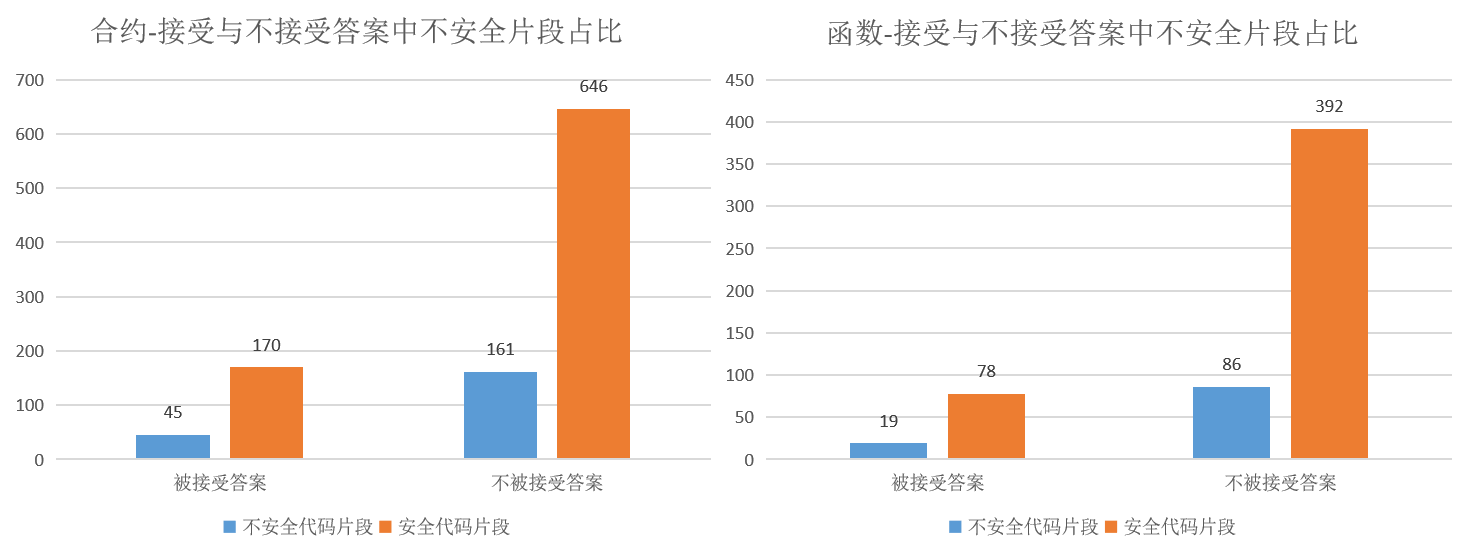
\includegraphics[width=1\textwidth]{figures/acceptedAns.png}
\caption{被接受答案与不被接受答案的不安全帖子比例}
\captionsetup{font={footnotesize}}
\label{acceptedAns}
\end{figure}

本文探究了出现最频繁的Arithmetic漏洞的类型以及它的分布特点。从结果\ref{Arithmetic}来看,
Arithmetic漏洞在所有检测到的合约漏洞占比66\%,在所有检测到的函数漏洞占比64\%,主要为上下溢出漏洞。根据统计,Arithmetic漏洞在73\%的包含合约的代码片段与78\%的包含函数的代码片段中存在。

%todo 图错了 改成占比
\begin{figure}[htbp]
\centering
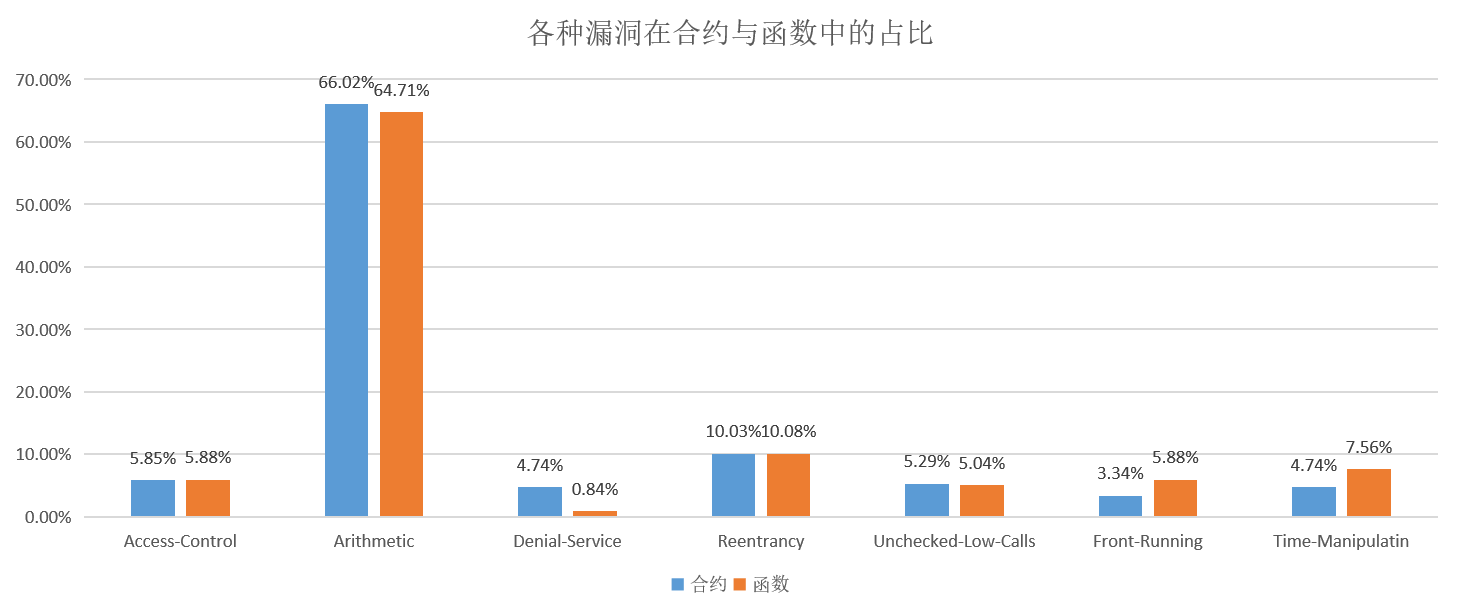
\includegraphics[width=1\textwidth]{figures/bugCount.png}
\caption{各种漏洞在合约与函数中的占比}
\captionsetup{font={footnotesize}}
\label{Arithmetic}
\end{figure}

本文发现StackOverflow智能合约代码片段中的11.91\%的代码片段包含漏洞;主要的漏洞类型是Arithmetic,它在大部分存在漏洞的代码片段中出现;最后,被接受的答案也并非安全。

\textbf{研究问题四:在 StackOverflow 中存在多少 Gas 低效模式?}

根据合约与函数的相似克隆对,本文获得了StackOverflow上Gas低效模式的分布,结果如表\ref{gasPic}所示。

本文发现32.14\%(360/1120)的合约代码片段存在低效代码,13.46\%(82/609)的函数代码片段存在低效代码,总共25.56\%的代码片段包含至少一个Gas低效模式。总共在合约代码片段找到459个低效模式,在函数代码片段找到86个低效模式。

这个结果相较于漏洞的比例,在合约代码片段中达到了32.14\%,这可能是由于是Gas智能合约进行交易时的费用,是随着智能合约产生的新概念,Gas低效模式是一种相较漏洞危害较小的缺陷。对编程人员而言更难套用其他语言的编程经验,也更容易忽视Gas低效模式。

\begin{table}[ht]
\centering

\begin{tabular}{cccccccc}
\hline
低效模式类型 & Pattern1 & Pattern2 & Pattern3 & Pattern4 & Pattern5 & Pattern6 & 总计  \\ \hline
合约     & 70       & 249      & 8        & 6        & 29       & 11       & 459 \\
函数     & 2        & 69       & 1        & 1        & 11       & 2        & 86  \\ \hline
总计     & 72       & 318      & 9        & 7        & 40       & 13       & 545 \\ \hline
\end{tabular}
\caption{StackOverflow的Gas低效模式分布}
\label{gasPic}
\end{table}

总体来看,能找到的最多的低效模式是Pattern2,编程人员倾向于使用Gas低效的变量类型与变量定义顺序。在合约与函数层面上,Pattern1区别较大,这是因为Pattern1与变量定义有很大关系,只有在出现较多的变量定义时,才有较大可能出现Pattern1。根据本文的随机抽查,在Pattern1中存在变量定义的函数并不会定义较多的局部变量。
%根据本文的统计,在50个函数中,23个函数存在变量定义,然而它们的平均变量定义数仅为1.3。

对于Pattern3与Pattern4,它们的数量较少,这与Kong等\cite{gasPattern}的结果接近,考虑到Pattern3是寻找对合约层面上全局变量的无意义赋值,在函数克隆对上没有任何结果是合理的。

对于Pattern4,虽然本文已经对工具的返回信息做处理,仅使用变量调用时的位置信息,然而在工具论文中Pattern4的检测数量较低,本文认为是这种写法在智能合约开源项目与StackOverflow的问题讨论中并没有广泛的出现。

Pattern5指的是不满足短路规则的条件判断语句对Gas消耗产生的影响,本文发现这部分的低效模式检测结果与代币合约相关度较大,如图\ref{pattern5-example}所示代码,合约持有者使用frozen变量决定代币合约是否暂停交易;如果在持有者已经暂停交易,提前判断frozen == false将会使用更少的字节码。

\begin{figure}[htbp]
\centering
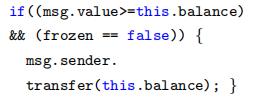
\includegraphics[width=0.4\textwidth]{figures/pattern5-example.png}
\caption{Pattern5例子}
\captionsetup{font={footnotesize}}
\label{pattern5-example}
\end{figure}

对于Pattern6,本文检查了所有的克隆对,确定是否存在来自开源项目的合约或函数存在Pattern6而来自StackOverflow的代码片段没有,检验表明由于本文要求“Modifiers”序列一致,所有检测到Pattern6的克隆对在Pattern6上保证了低效模式定位的一致性。



%todo 解释Gas估计
对于每种Gas低效模式,根据GPFinder的重放实验,获得了Gas低效模式在合约部署时的额外Gas消耗,本文将其作为一种Gas低效模式的Gas消耗估计。

图\ref{gasGuess}结果表明,Pattern1、Pattern2、Pattern5影响最为严重,并且函数代码片段的Gas消耗估计远低于合约代码片段。

\begin{figure}[hb]
\centering
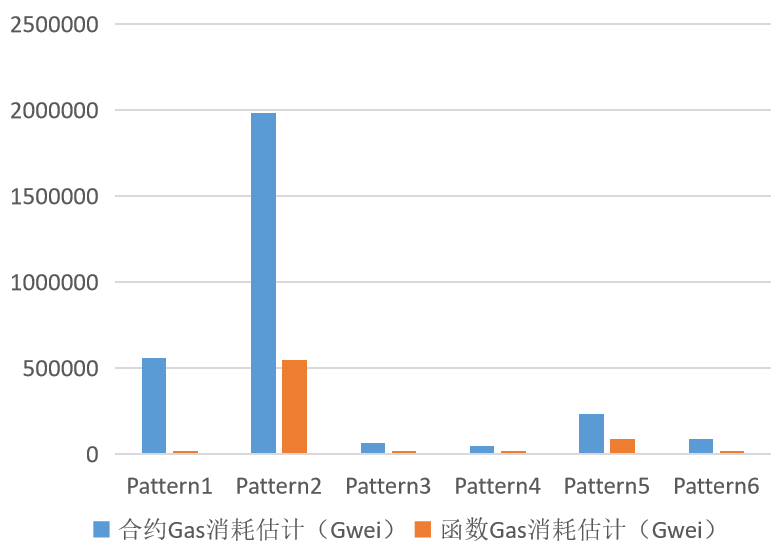
\includegraphics[width=0.8\textwidth]{figures/gasGuess.png}
\caption{StackOverflow上合约与函数的Gas消耗估计}
\captionsetup{font={footnotesize}}
\label{gasGuess}
\end{figure}

本文发现:StackOverflow智能合约的25.56\%的代码片段包含至少一个Gas低效模式,最主要的Gas低效模式与变量定义类型与变量定义顺序有关。

\textbf{研究问题五:来自 StackOverflow 的漏洞与Gas低效模式在开源智能合约中的普遍程度?}

%研究问题3的结果1
\begin{figure}[ht]
\centering
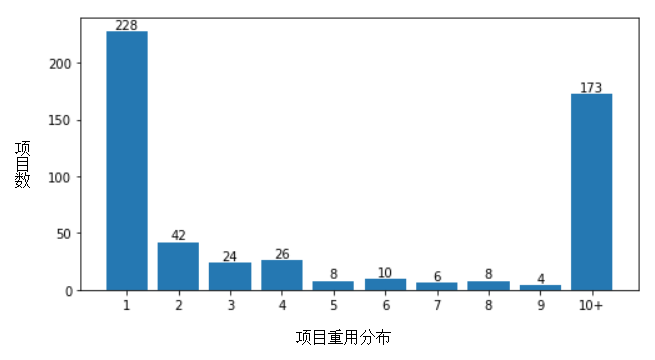
\includegraphics[width=0.8\textwidth]{figures/proli_result.png}
\caption{重用合约分布}
\captionsetup{font={footnotesize}}
\label{reuse_distribution}
\end{figure}

本文总共获得了 1120 个合约层面匹配对,这些匹配对对应于来自 开源项目库 的453 个开源项目中的529个合约。

%研究问题3的结果2
\begin{table*}[hbp]
\centering

\resizebox{\textwidth}{!}{%
\begin{tabular}{ccccccccc}
\hline
漏洞类型   & Access-Control & Arithmetic & Denial-Service & Reentrancy & Unchecked-Low-Calls & Front-Running & Time-Manipulation & 总计 \\ \hline
Mythril & 8     & 3895  & 0   & 1053 & 0     & 59 & 0  & 5015  \\
Osiris  & 0     & 46183 & 10  & 3    & 0     & 0  & 13 & 46209 \\
Slither & 35    & 0     & 781 & 48   & 205   & 0  & 8  & 1077  \\ 
总计      & 43    & 50078 & 791 & 1104 & 205   & 59 & 21 & 52301 \\ \hline
低效模式类型 & Pattern1       & Pattern2   & Pattern3       & Pattern4   & Pattern5            & Pattern6      &                   & 总计 \\ \hline
总计      & 31203 & 29747 & 24  & 21   & 17487 & 45 &    & 78527 \\ \hline
\end{tabular}
}
\caption{重用项目下的漏洞与Gas低效模式分布}
\label{pro_bug}
\end{table*}

图 \ref{reuse_distribution} 显示了 529 个项目的复用程度。

%重用10次以上的项目占比较高,为66.0\%,其次是重用1次的项目,16.3\%,从1次下降到9次。共有 530 份项目被重复使用两次以上,所有项目的平均重复次数为 1,364。

重用1次的合约占比较高,为43.10\%,其次是复用10次以上的合约,为32.70\%,总共有56.90\%的合约被复用了两次以上,所有项目的平均重复次数为1,364,这意味着开源项目之间已经存在严重的复用。

在17万的开源项目中,25.2\%至少包含一个StackOverflow的代码片段,6.7\%包含至少一个不安全的代码片段,16.1\%包含至少一个Gas低效的代码片段。

\begin{figure}[hb]
\centering
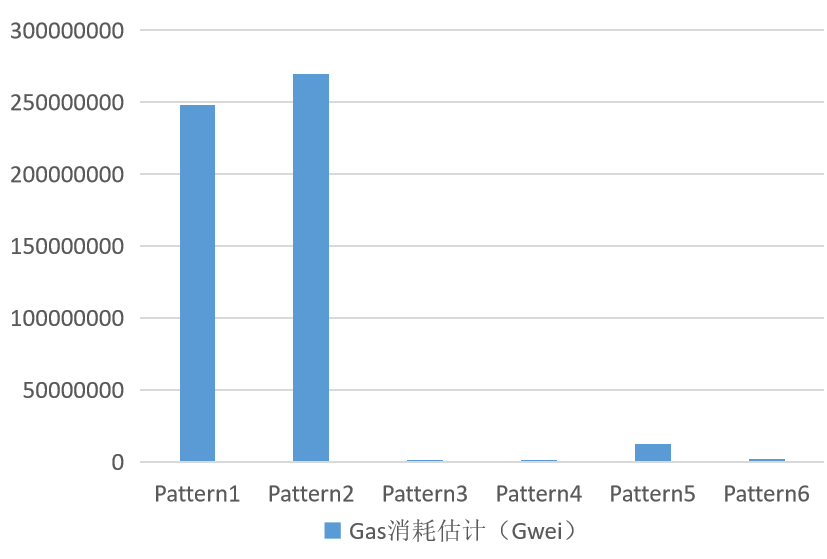
\includegraphics[width=0.6\textwidth]{figures/openResourceGas.png}
\caption{在开源项目扩散的Gas低效模式的Gas消耗估计}
\captionsetup{font={footnotesize}}
\label{gasDistributionGuess}
\end{figure}

表 \ref{pro_bug} 显示了这些错误在实际智能合约中的普遍性。
本文可以看到最常见的错误是Arithmetic、Denial-Service与Reentrancy。此外,Access-Control、Time-Manipulation、Front-Running 发生的频率相对较低,这些 漏洞 的数量分别为 43 和 21 和 59。

对于Gas低效模式,本文发现即使在扩散情况下,Pattern3、Pattern4、Pattern6都没有明显的扩散趋势。

Gas消耗估计结果\ref{gasDistributionGuess}显示,Pattern1、Pattern2与Pattern5扩散严重,由于Pattern5对Gas消耗较低,它产生的影响相较更低。

本文发现:智能合约本身复用程度较高,并且智能合约与StackOverflow代码片段的代码克隆程度同样较高;扩散的Gas低效模式比例较高,达到16.1\%,其中影响较大的为Pattern1与Pattern2。

StackOverflow中的漏洞与Gas低效模式确实的存在于这些复用开源项目中。如果 StackOverflow上的智能合约出现漏洞,很可能会影响到真正的智能合约。

\section{本章小结}

本章是在第二章和第三章的理论研究的基础上,对抽象语法树的代码克隆方法在问答网站实证研究中的有效性与问答网站上漏洞与Gas低效模式分布的结果评估。本文首先使用BLEU筛选了高BLEU的代码匹配对用于验证BLEU是否能够作为代码相似的指标,并且建立了验证数据集。本文使用了基于抽象语法树的代码克隆方法找到了合约与函数层面的代码克隆对,本文还验证了这些克隆对是否能够保证漏洞与Gas低效模式的一致性既查准率以及其在验证集的查全率。

在实证研究部分,本文对StackOverflow的代码片段进行了大规模的检测,找到了一定数量的漏洞与Gas低效模式,并且探究了出现在StackOverflow的漏洞与Gas低效模式是否同样存在于开源项目中。

本文发现小结如下:
\begin{itemize}
    \item StackOverflow智能合约代码片段中的11.91\%的代码片段包含漏洞;主要的漏洞类型是Arithmetic;即使是被接受的答案也并非安全。
    \item StackOverflow智能合约的25.56\%的代码片段包含至少一个Gas低效模式,最主要的Gas低效模式与变量定义类型与变量定义顺序有关。
    \item 智能合约本身复用程度高;开源项目中,25.2\%至少包含一个StackOverflow的代码片段,6.7\%包含至少一个不安全的代码片段,16.1\%包含至少一个Gas低效的代码片段。
\end{itemize}
